\chapter{Interpretable Time Series Classification}\label{chapter_sax_vsm}

\textit{In this chapter I show a novel algorithm for interpretable time-series classification based on characteristic 
patterns discovery. }

\section{Introduction}
Time series classification is an increasingly popular area of research, providing solutions to a wide range of fields, 
including data mining, image and motion recognition, environmental sciences, health care, and chemometrics. 
Within the last decade, many time series representations, similarity measures, and classification algorithms were 
proposed following the rapid progress in data collection and storage technologies \cite{citeulike:10358271}. 
Nevertheless, to date, the best overall performing classifier in the field is the nearest-neighbor algorithm (1NN), 
that can be easily tuned for a particular problem by choosing either a distance measure, an approximation technique, 
or smoothing \cite{citeulike:10358271}.
The 1NN classifier is simple, accurate and robust, depends on a very few parameters 
and requires no training \cite{citeulike:10358271}, \cite{citeulike:532340}, \cite{citeulike:12563424}.
However, the 1NN technique has a number of significant disadvantages, where the major shortcoming is the 
inability to offer any insight into the classification results. Another limitation is its need for a significantly large 
training set representing a within-class variance in order to achieve desired accuracy. 
Finally, while having trivial initialization, 1NN classification is computationally expensive. 
Thus, the demand for an efficient and \textit{interpretable} classification technique capable of processing of large 
data volumes remains.

In this thesis, I propose an alternative to 1NN algorithm that addresses aforementioned limitations. 
In particular, the proposed technique provides a superior interpretability, learns efficiently from a small training set,
and has a low classification computational complexity. As I shall show in the following chapters, these algorithm's
properties, make it the best choice for the problem of recurrent behaviors discovery from software process artifacts trails.

\section{Prior and related work} \label{sax_vsm_prior}
Almost all of the existing techniques for time series classification can be divided in two major categories \cite{citeulike:11796594}. 
The first category includes techniques based on shape-based similarity metrics where distance is measured directly between time 
series points. Classical examples from this category is 1NN classifier built upon Euclidean distance \cite{citeulike:4214336} and 
DTW \cite{citeulike:3496861}. The second category consists of classification techniques based on structural similarity metrics, 
which employ a high-level representations of time series based on their global or local features. 
Examples from this category include classifiers based on time series representation obtained with DFT \cite{citeulike:5094223} or 
Bag-Of-Patterns \cite{citeulike:10525778}. 
The development of these distinct categories can be explained by the difference in their performance: 
while shape-based similarity methods are virtually unbeatable on short pre-processed time series \cite{citeulike:532340}, 
they usually fail on long and noisy data, where structure-based solutions demonstrate a superior performance \cite{citeulike:10525778}. 

Two techniques, relevant to my work, were recently proposed as possible alternatives to these two categories.Monoprice Enhanced Bas
The first is the Time Series Shapelet technique which features a superior interpretability and a compactness of delivered solution 
\cite{citeulike:7344347}. A Shapelet is a short time series ``snippet'' that is a representative of class
membership and is used for a decision tree construction facilitating class identification and interpretability.
In order to find a branching shapelet, the algorithm exhaustively searches for a best discriminatory shapelet on data split 
via an information gain measure. The algorithm's classification is built upon the similarity measure between a branching 
shapelet and a full time series, defined as a distance between the shapelet and a closest subsequence in the series 
when measured by the normalized Euclidean distance. This exact technique, potentially, combines the superior precision of 
exact shape-based similarity methods, and the high-throughput classification capacity of feature-based approximate techniques. 
However, while demonstrating a superior interpretability, robustness, and similar to 1NN algorithm performance, shapelets-based 
technique is computationally expensive, $O(n^{2}m^{3})$, where $n$ is a number of objects and $m$ is the length of a longest 
time series, making its adoption for many-class classification problems difficult\cite{citeulike:11345338}. 
While the better solution was recently proposed ($O(nm^{2})$), it is an approximate solution based on indexing \cite{citeulike:12563493}.

The second technique with interpretable results is 1NN classifier built upon the Bag-Of-Patterns (BOP) representation of time series 
\cite{citeulike:10525778}, which is equated to an Information Retrieval (IR) ``bag of words" concept 
and is obtained by extraction, transformation with Symbolic Aggregate approXimation (SAX) \cite{sax}, and counting the frequencies
of short overlapping subsequences (patterns) along the time series.
By applying this procedure to a training set, the algorithm converts the data into the vector space, where the original time series are 
represented by a pattern (SAX word) occurrence frequency vector. These vectors are classified with 1NN classifier built with Euclidean 
distance or Cosine similarity applied to raw frequencies or their $\text{\textbf{tf}}\ast\text{\textbf{idf}}$ weighting. 
It was shown that BOP has several advantages: its complexity is linear ($O(nm)$), it is rotation-invariant and considers local and 
global structures simultaneously, and it provides an insight into patterns distribution through frequency histograms.
The authors concluded, that the best classification accuracy of BOP-represented time series is achieved by using 1NN classifier based 
on Euclidean distance. 

I propose the algorithm that is called \mbox{SAX-VSM} that has similarities to the aforementioned techniques. 
Similar to shapelets-based approaches, the algorithm discovers time series subsequences which are characteristic representatives of a 
class, that enables a superior interpretability. 
However, instead of recursive search for class-discriminating shapelet, it ranks by “importance” all potential candidate subsequences 
\textit{at once} with a \textit{linear computational complexity} of $O(nm)$.
To achieve this, similarly to BOP, \mbox{SAX-VSM} converts all training time series into bags of SAX words and relies $\text{\textbf{tf}}\ast\text{\textbf{idf}}$ 
weighting and Cosine similarity for classification. Nonetheless, instead of building $n$ bags for each of the training time series, 
it builds a \textit{single bag of words for each of the classes}, that effectively provides a compact solution of $N$ weight vectors 
($N$ is the number of classes, typically $N<<n$), and a fast classification time of $O(m)$.

As I shall show, these distinct features - the generalization of the class' patterns with a single bag and their weighting - allow 
SAX-VSM to achieve a high classification accuracy and to provide an exceptional interpretability.

\section{Preliminaries}
Before describing the algorithm, I define the key terms for this section.
\begin{defn}\label{def_timeseries}
Formally speaking, a \textbf{\textit{Time Series}} is an ordered sequence of pairs \linebreak
\mbox{$T=((p_{1},t_{1}),(p_{2},t_{2}),...,(p_{i},t_{i}),...,(p_{m},t_{m}))$} where $p_{i} \in \mathbf{R^{n}}$
and timestamps are ordered \linebreak 
$t_{1} < t_{2} < ... < t_{i} <...<t_{m}$ and possibly not equidistant, i.e. $|t_{i}-t_{i-1}| \neq |t_{i}-t_{i+1}|$.
\end{defn}
However, in the research literature, without the loss of generality, the equispaced data is typically considered.
It is assumed, that usually, the raw time series can be trated (massaged, curated, interpolated) in order to become equispaced.
%\begin{defn}\label{def_tsdatabase}
%A \textbf{\textit{Time Series Database}} $D$ is an unordered collection (a set) of $n$ time series which are possibly of a different 
%length.
%\end{defn}

\begin{defn}\label{def_subsequence}
A time series \textbf{\textit{subsequence}} of length $k$ of a time series $T = (t_{1}, t_{2},...,t_{m})$ of length $m$ is a time 
series $T_{i,k} = (t_{i},t_{1+1},...,t_{i+k-1})$  where $1 \leq i \leq m - k + 1$, i.e. a contiguous subsequences of the time series.
\end{defn}

As discussed in Section \ref{section_numerosity_reduction}, SAX-VSM is built upon the bag-of-words representation of time
series which are obtained from \textit{overlapping subsequences}. Usually, overlapping subsequences are extracted with the 
\textit{sliding window} as shown at the Figure \ref{fig:sliding_window} \cite{citeulike:3977965} \cite{citeulike:3175749}.

\begin{figure}[tbp]
   \centering
   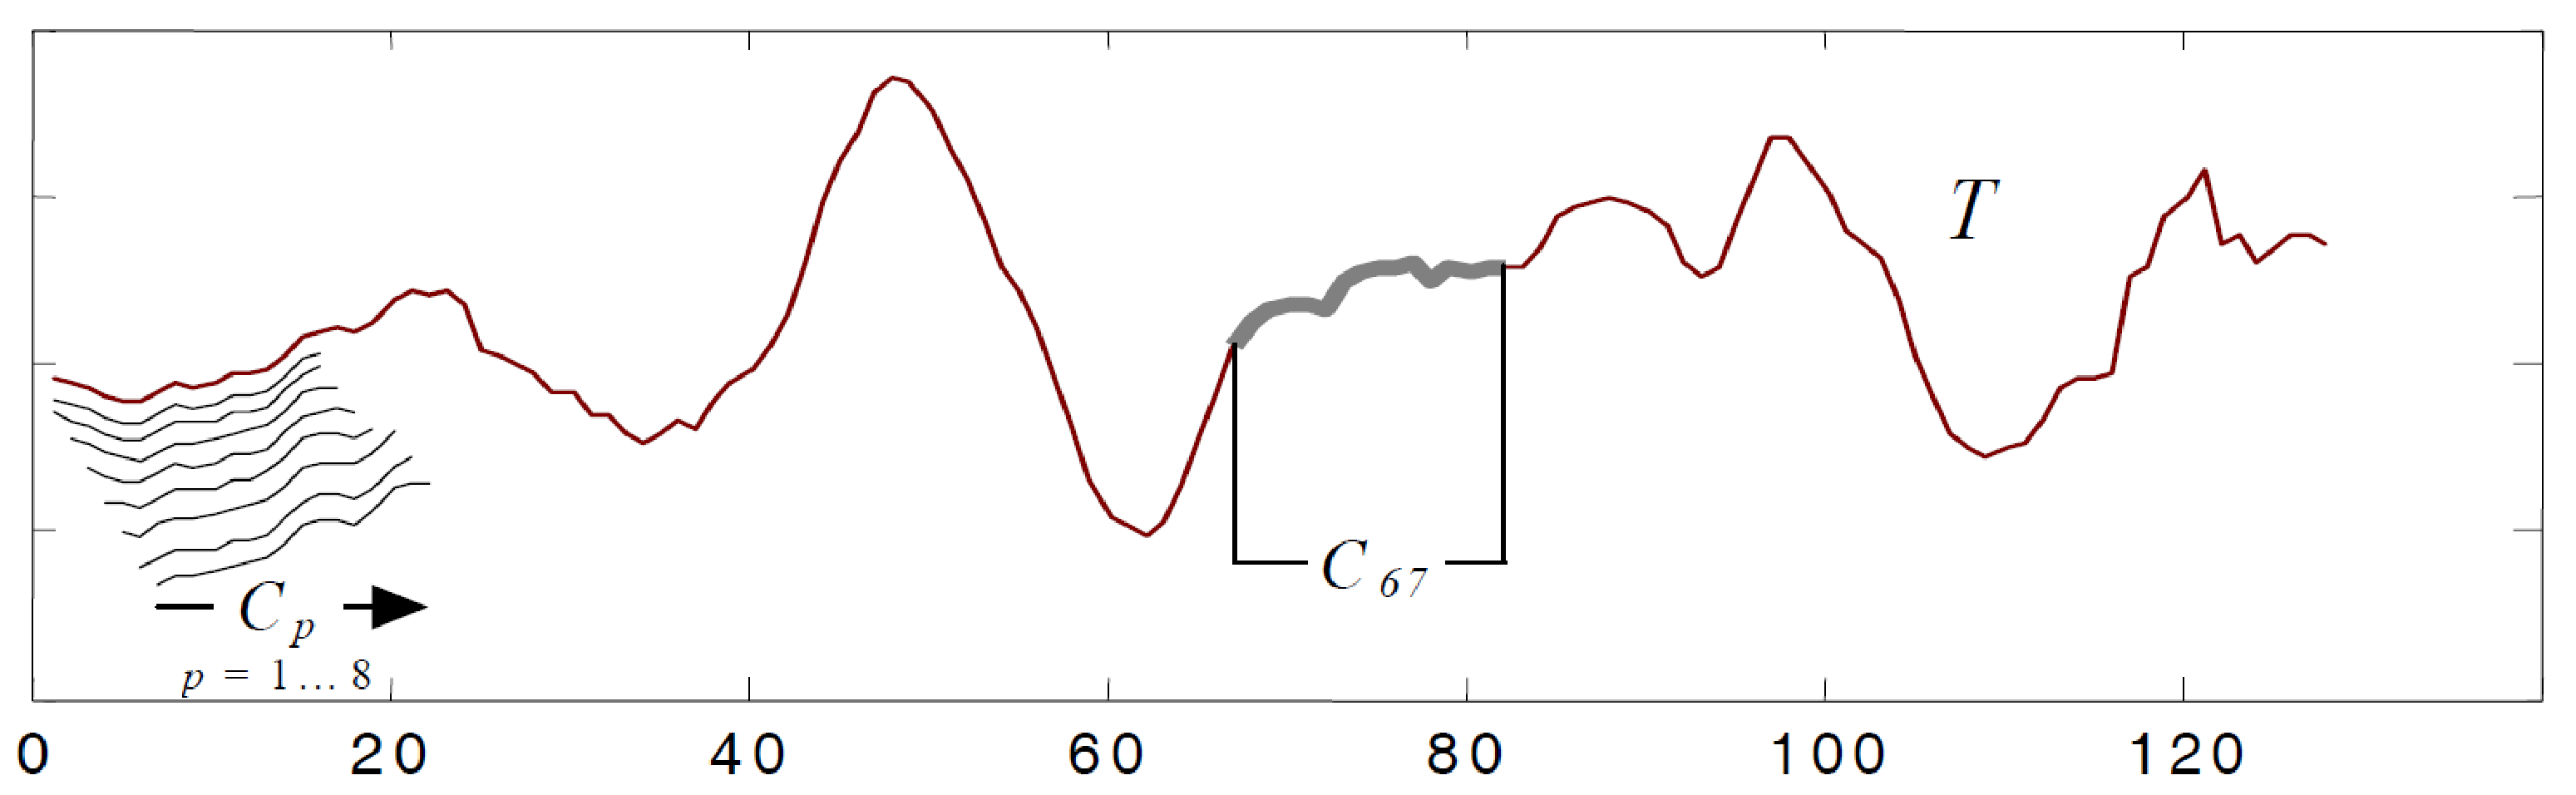
\includegraphics[height=45mm]{sliding-window.eps}
   \caption{An illustration of the sliding window technique from \cite{citeulike:2821475}: a time series T of length 128, 
   the subsequence $C67$ (of length $m$=16), and the first 8 overlapping subsequences extracted by a sliding window.}
   \label{fig:sliding_window}
\end{figure}

\section{SAX-VSM classification algorithm} \label{sax_vsm_background}
SAX-VSM is based on two well-known techniques. The first technique is Symbolic Aggregate approXimation, which is a high-level symbolic
representation of time series \cite{sax}. The second technique is Vector Space Model based on $\text{\textbf{tf}}\ast\text{\textbf{idf}}$
weighting scheme \cite{citeulike:300428}. 
Using SAX, the algorithm transforms real-valued time series classes into collections of SAX words. 
Next, by utilizing $\text{\textbf{tf}}\ast\text{\textbf{idf}}$ weighting, it transforms these collections into class-characteristic weight 
vectors, which, in turn, are used in the classification built upon Cosine similarity.

SAX, however, requires two parameters to be provided as an input and no efficient solution for their selection exists to the best of my knowledge. 
In this work I address this issue by using cross-validation and the parameters optimization scheme based on the dividing rectangles (DIRECT) 
algorithm that does not require any input \cite{citeulike:12563460}. 
DIRECT is a derivative-free optimization process that possesses local and global optimization properties; converges relatively quickly, and yields 
a deterministic, optimized solution. While other optimization techniques exist and some of them may perform better, the performance 
evaluation of the parameters selection is beyond the scope of my current work.

In the following subsections, I will review algorithms which are embedded in SAX-VSM. 
Subsection \ref{section-sax} reviews SAX - a symbolic discretization technique, 
Subsection \ref{section_numerosity_reduction} discusses numerosity reduction strategies,
Subsection \ref{bow_representation} reviews bag of words abstraction, 
terms weighting and Vector Space Model are discussed in the Subsection \ref{vsm}. 


\section{Symbolic Aggregate approXimation (SAX)}\label{section-sax}
Discretization of real data into a small number of finite values is highly desirable and sometimes required for machine learning 
algorithms. In addition, an effective dimensionality reduction is often vital for the ability to process datasets reflecting 
many real life phenomenas. Thus, probably hundreds of techniques currently developed and available for researchers dealing 
with knowledge discovery from variety of measurements.

Among these techniques, symbolic representation of time series attracting much attention by enabling the application of numerous 
string-processing algorithms, bioinformatics tools, and text mining techniques to time series \cite{sax}. 
The method provides a significant reduction of the time series dimensionality and a low-bounding to Euclidean distance 
metrics, which guarantees no false dismissal \cite{citeulike:2821475}. 
These properties are often leveraged by many time series analysis techniques which embed SAX representation for indexing and 
approximation. For example, adoption of SAX indexing allowed significant improvement in shapelet discovery speed in Fast-Shapelets 
algorithm \cite{citeulike:12563493} (but made the algorithm approximate). 

Given a time-series $T$ of a length $n$, SAX produces its symbolic approximation $\hat{S}$ of a length $w$ where letters are taken 
from an alphabet $\alpha$. Along with $T$, two parameters must be specified as the input: the alphabet size $\alpha$ and the size of 
the word to produce $w$. Algorithm works as follows. 

\begin{figure}[tbp]
   \centering
   \includegraphics[height=45mm]{sax_intro}
   \caption{An illustration of the SAX approach taken from \cite{citeulike:2821475} depicts two pre-determined breakpoints for the 
   three-symbols alphabet and the conversion of the time-series of length $n=128$ into PAA representation followed by mapping of 
   the PAA coefficients into SAX symbols with $w=8$ and $a=3$ resulting in the string \textbf{baabccbc}.}
   \label{fig:sax_intro}
\end{figure}

At first, since it is meaningless to compare time series with different offsets and amplitudes \cite{citeulike:532340} the time series 
$T$ is normalized to unit of standard deviation. This normalization procedure, also known as \textit{z-normalization} or 
``normalization to Zero Mean and Unit of Energy'', allows to minimize the effect of the time series amplitude while preserving time 
series structural specificities \cite{citeulike:3815880}. In order to obtain the normalized time series $\widetilde{T}$, the 
input time series mean is subtracted from each point and the resulted value is divided by standard deviation:
\begin{equation}
\Large
\widetilde{t}_{i} = \frac{x_{i}-\mu}{\sigma}, i \in {1,..,n}
\label{eq:znorm}
\end{equation}
If, however, the standard deviation value falls below a fixed threshold, the normalization procedure is not applied in order to avoid 
possible over-amplification of a background noise - as shown in \cite{citeulike:2821475}.

At the second step, the dimensionality of the normalized time series is reduced to $w$ by obtaining its 
Piecewise Aggregate Approximation (PAA). The PAA transforms the normalized time series $\widetilde{T}$ into a vector 
of PAA coefficients $C$ ($|C|=\omega$) by dividing it into equal-sized segments and computing their mean values:
\begin{equation}
\Large
c_{i} = \frac{w}{n} \sum_{j=\frac{n}{w}(i-1)+1}^{\frac{n}{w}i} \widetilde{x}_{j}
\label{eq:paa}
\end{equation}
It was shown by Keogh et al. \cite{citeulike:3000416} for PAA and by Yi \& Faloutsos \cite{citeulike:2946589} for any $L_{p}$ norm,
that this transformation satisfies to a bounding condition and guarantees no false dismissals.

Discretization is performed at the final step of SAX algorithm. Each of the PAA representation coefficients obtained at the previous step 
is converted into a letter $\widehat{c}$ of the alphabet $\alpha$ of the size $a$ by the use of lookup tables (\ref{sax_table}) which define a 
list of breakpoints $B=\beta_{1}, \beta_{2}, ... , \beta_{a-1}$ such that $\beta_{i-1} < \beta_{i}$ and $\beta_{0} = -\infty$, $\beta_{a} = \infty$ 
that divide the area under $N(0,1)$ into $a$ equal areas. The design of these tables rests on the assumption that normalized series tend to have 
Gaussian distribution \cite{citeulike:10141990}.
By assigning a corresponding alphabet symbol $alpha_{j}$ to each interval $[\beta_{j-1},\beta_{j})$, the conversion of the vector of PAA coefficients 
$C$ into the string $\widehat{C}$ implemented as follows: 
\begin{equation}
\Large
\widehat{c}_{i} = alpha_{j}, \; \text{iif} \; \bar{c}_{i} \in [\beta_{j-1},\beta_{j})
\label{eq:sax_alphabet}
\end{equation}

\begin{table}[t]
 \caption{An example of the SAX alphabet lookup table that contains the breakpoints dividing a Gaussian distribution in an arbitrary 
number (from 2 to 11) of equiprobable regions.}
 \label{sax_table}
 \small
\begin{tabularx}{\textwidth}{|l|X|X|X|X|X|X|X|X|X|X|}
\hline
\backslashbox{$\beta_{i}$}{$\alpha$} & 2 & 3 & 4 & 5 & 6 & 7 & 8 & 9 & 10 & 11 \\
\hline
$\beta_{1}$ & 0,00 & -0,43 & -0,67 & -0,84 & -0,97 & -1,07 & -1,15 & -1,22 & -1,28 & -1,34  \\
\hline
$\beta_{2}$ &\cellcolor{gray!25}& 0,43 & 0,00 & -0,25 & -0,43 & -0,57 & -0,67 & -0,76 & -0,84 & -0,91  \\
\hline
$\beta_{3}$ &\cellcolor{gray!25}&\cellcolor{gray!25}& 0,67 & 0,25 & 0,00 & -0,18 & -0,32 & -0,43 & -0,52 & -0,60  \\
\hline
$\beta_{4}$ &\cellcolor{gray!25}&\cellcolor{gray!25}&\cellcolor{gray!25}& 0,84 & 0,43 & 0,18 & 0,00 & -0,14 & -0,25 & -0,35 \\
\hline
$\beta_{5}$ &\cellcolor{gray!25}&\cellcolor{gray!25}&\cellcolor{gray!25}&\cellcolor{gray!25}& 0,97 & 0,57 & 0,32 & 0,14 & 0,00 & -0,11  \\
\hline
$\beta_{6}$ &\cellcolor{gray!25}&\cellcolor{gray!25}&\cellcolor{gray!25}&\cellcolor{gray!25}&\cellcolor{gray!25}& 1,07 & 0,67 & 0,43 & 0,25 & 0,11 \\
\hline
$\beta_{7}$ &\cellcolor{gray!25}&\cellcolor{gray!25}&\cellcolor{gray!25}&\cellcolor{gray!25}&\cellcolor{gray!25}&\cellcolor{gray!25}& 1,15 & 0,76 & 0,52 & 0,35  \\ 
\hline
$\beta_{8}$ &\cellcolor{gray!25}&\cellcolor{gray!25}&\cellcolor{gray!25}&\cellcolor{gray!25}&\cellcolor{gray!25}&\cellcolor{gray!25}&\cellcolor{gray!25}& 1,22 & 0,84 & 0,60  \\
\hline
$\beta_{9}$ &\cellcolor{gray!25}&\cellcolor{gray!25}&\cellcolor{gray!25}&\cellcolor{gray!25}&\cellcolor{gray!25}&\cellcolor{gray!25}&\cellcolor{gray!25}&\cellcolor{gray!25}& 1,28 & 0,91  \\
\hline
$\beta_{10}$&\cellcolor{gray!25}&\cellcolor{gray!25}&\cellcolor{gray!25}&\cellcolor{gray!25}&\cellcolor{gray!25}&\cellcolor{gray!25}&\cellcolor{gray!25}&\cellcolor{gray!25}&\cellcolor{gray!25}& 1,34  \\
 \hline
\end{tabularx}
\vspace{0.1cm}
\end{table}

SAX introduces new metrics for measuring distance between strings by extending Euclidean and PAA (\ref{eq:paa_distance}) distances. 
The function returning the minimal distance between two string representations of original time series $\widehat{Q}$ and $\widehat{C}$ is defined as
\begin{equation}
\text{MINDIST}(\widehat{Q},\widehat{C}) \equiv \sqrt{ \frac{n}{w} } \sqrt{ \sum_{i=1}^{w} ( dist( \widehat{q}_{i}, \widehat{c}_{i} ) )^{2}}
\label{eq:sax_mindist}
\end{equation} 
where the $dist$ function is implemented by using the lookup table for the particular set of the breakpoints (alphabet size) as shown in 
Table \ref{tbl:sax_lookup}, and where the singular value for each cell $(r,c)$ is computed as 
\begin{equation}
cell_{(r,c)} = 
\begin{cases} 
0, \text{ if }\left| r-c \right| \leq 1 \\
\beta_{\max(r,c) - 1} - \beta_{\min(r,c) - 1}, \text{ otherwise}
\end{cases}
\label{eq:cell}
\end{equation}


\begin{table}
\caption{A lookup table used by the MINDIST function for the $a=11$}
\label{tbl:sax_lookup}
\small
\begin{tabularx}{\textwidth}{|l|X|X|X|X|X|X|X|X|X|X|X|}
\hline
&\textbf{a}&\textbf{b}&\textbf{c}&\textbf{d}&\textbf{e}&\textbf{f}&\textbf{g}&\textbf{h}&\textbf{i}&\textbf{j}&\textbf{k} \\
\hline
\textbf{a}& 0,00 & 0,00 & 0,43 & 0,73 & 0,99 & 1,22 & 1,45 & 1,68 & 1,94 & 2,24 & 2,67 \\
\hline
\textbf{b}& 0,00 & 0,00 & 0,00 & 0,30 & 0,56 & 0,79 & 1,02 & 1,26 & 1,51 & 1,82 & 2,24 \\
\hline
\textbf{c}& 0,43 & 0,00 & 0,00 & 0,00 & 0,26 & 0,49 & 0,72 & 0,95 & 1,21 & 1,51 & 1,94 \\ 
\hline
\textbf{d}& 0,73 & 0,30 & 0,00 & 0,00 & 0,00 & 0,23 & 0,46 & 0,70 & 0,95 & 1,26 & 1,68 \\ 
\hline
\textbf{e}& 0,99 & 0,56 & 0,26 & 0,00 & 0,00 & 0,00 & 0,23 & 0,46 & 0,72 & 1,02 & 1,45 \\ 
\hline
\textbf{f}& 1,22 & 0,79 & 0,49 & 0,23 & 0,00 & 0,00 & 0,00 & 0,23 & 0,49 & 0,79 & 1,22 \\ 
\hline
\textbf{g}& 1,45 & 1,02 & 0,72 & 0,46 & 0,23 & 0,00 & 0,00 & 0,00 & 0,26 & 0,56 & 0,99 \\ 
\hline
\textbf{h}& 1,68 & 1,26 & 0,95 & 0,70 & 0,46 & 0,23 & 0,00 & 0,00 & 0,00 & 0,30 & 0,73 \\ 
\hline
\textbf{i}& 1,94 & 1,51 & 1,21 & 0,95 & 0,72 & 0,49 & 0,26 & 0,00 & 0,00 & 0,00 & 0,43 \\ 
\hline
\textbf{j}& 2,24 & 1,82 & 1,51 & 1,26 & 1,02 & 0,79 & 0,56 & 0,30 & 0,00 & 0,00 & 0,00 \\ 
\hline
\textbf{k}& 2,67 & 2,24 & 1,94 & 1,68 & 1,45 & 1,22 & 0,99 & 0,73 & 0,43 & 0,00 & 0,00 \\ 
\hline
\end{tabularx}
\end{table}

As shown by Li et al., this SAX distance metrics lower-bounds the PAA distance, i.e.
\begin{equation}
\sum_{i=1}^{n} (q_{i} - c_{i})^{2} \geq n(\bar{Q} - \bar{C})^{2} \geq n(dist(\hat{Q},\hat{C}))^2
\label{eq:sax_bounding}
\end{equation}

The SAX lower bound was examined by Ding et al. \cite{citeulike:4501572} in great detail and was found 
to be superior in precision to the spectral decomposition methods on non-periodic data sets while only
``slightly'' inferior to other techniques on periodic data. This findings and the capacity of SAX to be
tuned for data specificities made it the best solution for symbolic discretization step of SAX-VSM.

\subsection{SAX discretization of time series}\label{sec_sax_representation}
One of the ways to represent the time series in symbolic form is to reduce the dimensionality and to 
discretize the whole time series. The drawback with this approach is that due to the rough approximation 
it often does not capture enough local details in the data, which severely affects many pattern discovery
techniques \cite{\cite{citeulike:10525778}}.  Another way to represent a time series is by a discretization 
of a collection of overlapping subsequences extracted with a sliding window. 

SAX-VSM relies on this sliding window technique to convert a time series $T$ of a length $m$ into 
the set of $k$ SAX words, where $k=(m-l_{s})+1$ and $l_{s}$ is the sliding window length. 
By sliding a window of length $l_{s}$ across time series $T$, extracting subsequences, 
converting them to SAX words, and placing these words into an unordered collection (a database), 
it obtains the \textit{bag of words} representation of the original time series $T$.

\subsection{Bag of words representation of time series}\label{bow_representation}
Following its introduction, SAX was shown to be an efficient tool for solving problems 
of finding motifs and discords in time series \cite{citeulike:3977965, citeulike:3175749}. 
The authors employed a sliding window-based subsequence extraction technique 
and augmented data structures (hash table in \cite{citeulike:3977965} and trie in \cite{citeulike:3175749}) 
in order to build SAX words ``vocabularies''. Further, by analyzing words frequencies 
and locations, they were able to capture frequent and rare SAX words representing 
motifs and discords subsequences. Later, the same technique based on the combination 
of sliding window and SAX was used in the numerous works, most notably in time series 
classification using bag of patterns (BOP) \cite{citeulike:10525778}. 

I also use this sliding window technique to convert a time series $T$ of a length $n$ into 
the set of $m$ SAX words, where $m=(n-l_{s})+1$ and $l_{s}$ is the sliding window length. 
By sliding a window of length $l_{s}$ across time series $T$, extracting subsequences, 
converting them to SAX words, and placing these words into an unordered collection, 
the algorithm builds the \textit{bag of words} representation of the original time series $T$.

\subsection{SAX numerosity reduction}\label{section_numerosity_reduction}
Previously, the analysis of the SAX-based algorithms performance revealed that the best matches for an extracted 
by sliding window subsequence tend to be its immediate neighbors, in particular the subsequence one point to the 
right and the subsequence one point to the left \cite{citeulike:3977965} \cite{citeulike:3175749}, 
due to the smoothing effects of PAA approximation and SAX discretization \ref{section-sax}. 
The authors defined these matching subsequences as the \textit{trivial matches} and found that in the smooth 
regions of the time series, the amount of trivial matches can be large enough to dominate over true patterns due to 
over-counting, which may not only distort results, but could make them meaningless \cite{citeulike:227029}. 
Therefore, they concluded, when extracting subsequences from the time series by a sliding window, the trivial 
matches should be excluded. 

The authors proposed a sampling strategy based on a \textit{MINDIST} \ref{eq:sax_mindist} distance 
function designed in order to avoid the ``trivial and degenerate solutions'': if $l$ consecutive SAX words \newline 
$\widehat{S}_{i,k}, \widehat{S}_{i+1,k},...,\widehat{S}_{i+l-1,k},...$
corresponding to subsequences $T_{i,k}, T_{i+1,k},...,T_{i+l-1,k},...$ extracted with sliding window are 
equal when using \textit{MINDIST}, they kept only the first entry $\widehat{S}_{i,k}$. 
They further argued, that similarly to the run length encoding data compression techniques, if one would 
ever need to retrieve all the occurrences of $\widehat{S}_{i,k}$, they can be found by sliding the window from 
the first occurrence to the right until the word which is different from $\widehat{S}_{i,k}$ is found. 
While the authors found the inclusion of the numerosity reduction vital for motif and discords discovery, 
intuitively, in the case of SAX-VSM, the over-counting effect is significantly mediated by the design of 
$\text{\textbf{tf}}\ast\text{\textbf{idf}}$ statistics \eqref{formula:tfidf}. 
Moreover, the exclusion of ``trivial matches'' may degrade the overall performance of bag of words based 
approach, as it was shown in \cite{citeulike:10525778}.

In order to clarify this issue, I have conducted a series of experiments for three numerosity reduction strategies 
\ref{nr_study} and found, that for most of the data sets, the use of the numerosity reduction significantly reduces 
DIRECT scheme convergence time and improves its accuracy. 
Furthermore, once I have relaxed the trivial match constraints by substitution of \textit{MINDIST} distance function 
with Hamming distance \cite{hamming}, I was able to improve the classification accuracy for more than half of the data 
sets that I have used for SAX-VSM performance evaluation (see \cite{jmotif}). 

The \textit{HAMMING} distance function for two SAX words $\hat{Q}$ and $\hat{C}$ of the same length $w$ 
is defined as the number of letters in which they differ.
\begin{equation}
\label{eq:hamming}
\begin{split}
\text{HAMMING}(\widehat{Q},\widehat{C}) \equiv \sum_{i=1}^{w} I( \widehat{q}_{i}, \widehat{c}_{i} ), \\
\text{where } I( \widehat{q}_{i}, \widehat{c}_{i} ) = \begin{cases}
                                                       1,\text{ if } \widehat{q}_{i} \neq \widehat{c}_{i} \\
                                                       0,\text{ if } \widehat{q}_{i} = \widehat{c}_{i}
                                                      \end{cases}
\end{split}                                                      
\end{equation}

While constructing bag of words as explained in Section \ref{bow_representation},  SAX-VSM compares each newly 
extracted word to the last word added to the bag using \textit{HAMMING} distance function.
If these words appear to be equal, i.e. distance is zero, it discards the to be added word and continues as usual. 

For further use, I abbreviate the numerosity reduction strategy based on previous work and \textit{MINDIST} 
function as \textit{CLASSIC}, while the one based on \textit{HAMMING} distance as \textit{EXACT}.

\subsection{Vector Space Model (VSM) adaptation}\label{vsm}
I use Vector space model exactly as it is known in information retrieval (IR) \cite{citeulike:300428} for 
manipulations with abstracted by SAX words timeseries. 

Similarly to IR, define and use the following expressions:
\begin{itemize}
  \item \textit{term} - a single SAX word;
  \item \textit{bag of words} - an unordered collection of SAX words;
  \item \textit{corpus} - a set of bags;
  \item \textit{weight matrix} - a matrix defining weights of all words in a corpus.
\end{itemize}
Note however, that I use terms \textit{bag of words} and \textit{document} for abbreviation of an unordered 
collection of SAX words interchangeably, while in IR these usually bear different meaning: \textit{document} 
usually presumes certain words ordering (semantics). 
Although similar definitions, such as \textit{bag of features} \cite{citeulike:12636726} 
or \textit{bag of patterns} \cite{citeulike:10525778}, were recently proposed for techniques built 
upon SAX \cite{citeulike:10525778}, I use the traditional \textit{bag of words} definition since it reflects 
my workflow precisely. 

Given a training set of time series, SAX-VSM builds a bag of SAX words for each of its classes by processing 
each time series with a sliding window and SAX. Then, bags are combined into a corpus, which is built as a 
\textit{term frequency matrix}, whose rows correspond to the set of all SAX words (terms) 
found in \textit{all classes}, whereas each column denotes a class of the training set. 
Each element of this matrix is an observed frequency of a term in a class. 
Because SAX words extracted from the time series of one class are often not 
found in others, as shown in Section \ref{scalability}, this matrix is usually sparse. 
%Many elements of this matrix are zeros - because words extracted from one class 
%are often not found in others (Figure \ref{fig:venn}). 
%By its design, this sparse term frequency matrix is a dictionary of all SAX words extracted from all time 
%series of a training set, which accounts for frequencies of each word in each of 
%the training classes.

\begin{table}
\caption{The SMART notation. }
\vspace{0.4cm}
\label{tbl:smart}
\begin{tabularx}{\textwidth}{l l l}
\toprule[1pt]
\textbf{Term frequency} &\textbf{Document frequency} &\textbf{Normalization} \\[0.5ex]
\midrule
n (natural):  $\text{tf}_{t,d}$ & n (no): 1 & n (none): 1 \\[2ex]
l (logarithm): $1+log(\text{tf}_{t,d}$) & t (idf): $log\tfrac{N}{df_{t}}$ & c (cosine): $\tfrac{1}{\sqrt{w_1^2 + w_2^2 + ... + w_M^2}}$ \\[2ex]
a (augmented): $0.5 + \tfrac{0.5 \times \text{tf}_{t,d}}{\text{max(tf}_{t,d})}$ & p (prob idf): $\textbf{max}\left( 0,\text{log}\tfrac{N-df_{t}}{df_{t}} \right) $ & 
b (byte size): $\tfrac{1}{CharLength^\alpha}, \alpha < 1 $ \\[2ex]
b (boolean): $\begin{cases} 1, & \text{if tf}_{t,d} > 0 \\ 0, & \text{otherwise} \end{cases} $ & & \\[3ex]
L (log average): $ \tfrac{1+\text{log}(\text{tf}_{t,d})}{1+\text{log}(\text{ave}_{t \epsilon d}( \text{tf}_{t,d}))}$ & & \\[1ex]
\bottomrule[1pt]
\end{tabularx}
\end{table}

Following to the common in IR workflow, SAX-VSM employs the $\text{\textbf{tf}}\ast\text{\textbf{idf}}$ weighting scheme 
\cite{citeulike:4469058} for each element of this matrix in order to transform a frequency value into the 
weight coefficient. 
The $\text{\textbf{tf}}\ast\text{\textbf{idf}}$ weight for a term is defined as a product of two factors: term frequency ($\text{\textbf{tf}}$) 
and inverse document frequency ($\text{\textbf{idf}}$). 
For the first factor, I use logarithmically scaled term frequency (Table \ref{tbl:smart}) \cite{citeulike:4469058}:
\begin{equation}
 \mbox{\textbf{tf}}_{t, d} =  \begin{cases} \log(1 + \mbox{\textbf{f}}_{t,d}), &\mbox{if \textbf{f}}_{t,d}>0  \\
0, & \mbox{otherwise} \end{cases}
\end{equation} 
where $t$ is a term and $d$ is a bag of words (the document in IR terms), and $\mbox{\textbf{f}}_{t,d}$ 
is a frequency of the term in the bag.

For document frequency I use inverse document frequency:
\begin{equation}
 \mbox{\textbf{idf}}_{t, D} =  \log_{10}\frac{|D|}{|d \in D : t \in d|} = \log_{10}\frac{N}{\mbox{\textbf{df}}_{t}}
 \label{formula:idf}
\end{equation} 
where $N$ is the cardinality of corpus $D$ (the total number of classes) and the 
denominator $\mbox{\textbf{df}}_{t}$ is a number of documents where the term $t$ appears.

Thus, the $\text{\textbf{tf}} \ast \text{\textbf{idf}}$ value for a term $\text{\textbf{t}}$ in the document 
$\text{\textbf{d}}$ of a corpus $\text{\textbf{D}}$ is defined as:
\begin{equation}
 \text{\textbf{tf}} \ast \text{\textbf{idf}}(t, d, D) =  \text{\textbf{tf}}_{t, d} \times \text{\textbf{idf}}_{t, D} = \log(1 + \text{\textbf{f}}_{t,d})
\times \log_{10}\frac{N}{\mbox{\textbf{df}}_{t}}
 \label{formula:tfidf}
\end{equation} 
for the all cases where $\mbox{\textbf{f}}_{t,d}>0$ and $\mbox{\textbf{df}}_{t}>0$, or zero otherwise.
Once all terms of a corpus are weighted, the columns of a sparse matrix are used 
as \textit{class term weights vectors} that facilitate the classification using cosine similarity. 

Cosine similarity measure between two vectors is defined by their inner product and magnitude. 
For two vectors $\mathbf{a}$ and $\mathbf{b}$ that is:
\begin{equation}
%\mbox{similarity}(\boldsymbol{a},\boldsymbol{b}) = cos(\theta) = \frac{ \sum\limits^{n}_{i=1} a_{i}
%\times b_{i} }{
%\sqrt{\sum\limits^{n}_{i=1} a_{i}} \times \sqrt{\sum\limits^{n}_{i=1} b_{i}} }
\mbox{similarity}(\mathbf{a},\mathbf{b}) = cos(\theta) = 
\frac{ \mathbf{a} \cdot \mathbf{b} } {\left| \left| a \right| \right| \cdot \left| \left| b \right|\right|} =
\frac{ \sum\limits_{i=1}^{n}{a_{i} \times b_{i}} }{ \sqrt{\sum\limits_{i=1}^{n}{(a_{i})^2}} \times \sqrt{\sum\limits_{i=1}^{n}{(b_{i})^2}}}
\end{equation} 

\section{SAX-VSM classification algorithm} \label{sax-vsm}
As many other classification techniques, SAX-VSM consists of two phases - 
training and classification. 

\begin{figure}[t]
   \centering
   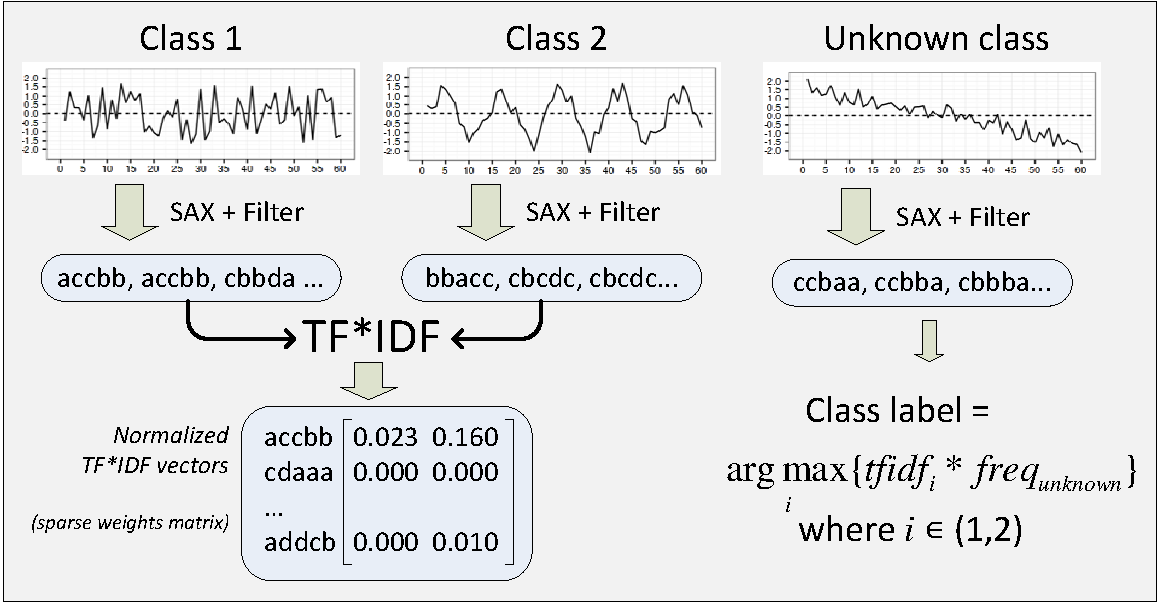
\includegraphics[width=148mm]{figures/overview.eps}
   \caption{
   An overview of SAX-VSM algorithm: 
   at first, labeled time series are converted into bags of words using SAX; 
   secondly, $\text{\textbf{tf}}\ast\text{\textbf{idf}}$ statistics is computed resulting in 
   a single weight vector per training class. For classification, an unlabeled 
   time series is converted into a term frequency vector and assigned a 
   label of a weight vector which yields a maximal cosine similarity value.
   This is \textit{ltc.nnn} weighting schema in SMART notation \ref{tbl:smart}.}
   \label{fig:sax-vsm_overview}
\end{figure}

\subsection{Training phase}
The training starts by transforming the labeled time series into SAX representation
configured by three parameters: the sliding window length (\textit{W}), 
the number of PAA segments per window (\textit{P}), 
and SAX alphabet size (\textit{A}).
Each of subsequences extracted with overlapping sliding window 
is normalized (Sec. \ref{section-sax}) before being processed with PAA. 
However, if the standard deviation value falls below a fixed threshold, the 
normalization is not applied in order to avoid over-amplification 
of a background noise \cite{sax}. 

By applying this procedure to all time series from $N$ training classes, 
algorithm builds a corpus of $N$ bags, to which it applies $\text{\textbf{tf}}\ast\text{\textbf{idf}}$ 
weighting and outputs $N$ real-valued weight vectors of equal length 
representing training classes. 

Because the whole training set must be processed, 
training of SAX-VSM classifier is computationally expensive ($O(nm)$). 
However, there is no need to maintain an index of training time series, 
or to keep any of them in the memory at the runtime;
the algorithm simply iterates over all training time series incrementally building 
bags of SAX words. Once built and weighted with $\text{\textbf{tf}}\ast\text{\textbf{idf}}$, 
the corpus is discarded - only a resulting set of $N$ real-valued weight vectors 
is retained for classification.

\subsection{Classification}
In order to classify an unlabeled time series, SAX-VSM transforms it into a
terms frequency vector using exactly the same sliding window technique 
and SAX parameters that were used for training. 
It computes cosine similarity values between this term frequency vector 
and $N$ $\text{\textbf{tf}}\ast\text{\textbf{idf}}$ weight vectors representing the training classes. 
The unlabeled time series is assigned to the class whose vector yields the
maximal cosine similarity value.

\section{Parameters optimization} \label{section-direct}
As shown above, SAX-VSM requires three discretization parameters to be specified upfront. 
Unfortunately, up to date, there is no efficient solution known for their selection to the best 
of my knowledge. In order to optimize the parameters selection while using only a training data, 
I propose a solution based on a common cross-validation and DIRECT (DIviding RECTangles) 
optimization scheme \cite{citeulike:4210208}. For brevity, I omit the detailed explanation 
of the algorithm, and refer the to \cite{citeulike:12563460} for additional details.

DIRECT is designed to deal with problems of form
\begin{equation}
 \min_{x} \: f(x) \text{, where } X_{L} \leq x \leq X_{U}
 \label{formula:direct}
\end{equation} 
where $f in \mathbf{R}$ and $x, X_{L}, X_{U} \in \mathbf{R}$. 

At the first step DIRECT scales the search domain to be the unit hypercube. The function is then evaluated 
at the center point of the hypercube. As pointed in \cite{citeulike:12563460}, computing the function value
at
the center is an advantage of the method when dealing with problems
in higher dimensions.
Then, DIRECT iteratively performs two procedures - partitioning the hypercube into smaller hyper-rectangles 
and identifying a set of potentially-optimal by sampling their centers. At each step, the function is evaluated 
at the center points of all potentially-optimal hyper-rectangles. Procedure continues interactively until the 
error function converges. DIRECT is guaranteed to converge to the global optimal function value,
as the number 
of iterations goes to infinity \cite{citeulike:12563460}.

Since DIRECT is designed to search for global minima of a real valued function over 
a bound constrained domain, I employ rounding of a reported solution values to the nearest integer.
Figure \ref{fig:direct-sampling} illustrates the application of leave-one-out cross-validation and DIRECT to 
\textit{SyntheticControl} data set, in this case, algorithm converged after sampling just 130 out of 13'860 
possible parameters combinations that is \textgreater100x speedup.

\begin{figure}[t]
   \centering
   \includegraphics[width=150mm]{figures/figure_direct.eps}
   \caption{Parameters optimization with DIRECT for \textit{SyntheticControl} dataset. 
   Left panel shows all points sampled by DIRECT in the space \mbox{$PAA*Window*Alphabet$},
   red points correspond to high error values while green points correspond to low error values 
   in cross-validation experiments. 
   Note the green points concentration at $W$=42. 
   Middle panel shows the classification error heat map obtained by a complete scan 
   of all 432 points of the hypercube slice when $W$=42. 
   Right panel shows the classification error heat map of the same slice when 
   the parameters search optimized by DIRECT, 
   the optimal solution ($P$=8,$A$=4) was found by sampling of 43 points.}
   \label{fig:direct-sampling}
\end{figure}


\section{Intuition behind SAX-VSM}
First, by combining \textit{\textbf{all}} SAX words extracted from 
\textit{\textbf{all}} time series of single class into a \textit{\textbf{single bag}} of 
words, SAX-VSM manages to capture and to ``generalize'' with PAA and SAX 
observed intraclass variability from a small training set.  

Secondly, by normalizing time series subsequences and by discarding their original 
ordering, SAX-VSM is capable to capture and to recognize characteristic 
subsequences in distorted and corrupted by noise or signal loss time series. 

Thirdly,  $\text{\textbf{tf}}\ast\text{\textbf{idf}}$ statistics naturally highlights terms unique to a
class by assigning them higher weights whereas terms observed in multiple classes are 
assigned weights inversely proportional to their interclass presence. This
improves the selectivity of classification by lowering a contribution of ``confusive'' 
multi-class terms, while increasing a contribution of class' ``defining'' terms to the
final similarity measure.

Ultimately, the algorithm compares a set of subsequences extracted from an unlabeled 
time series with a weighted set of all characteristic subsequences representing the whole 
of a training class. 
Thus, an unknown time series is classified by its similarity not to a given number of 
``neighbors'' (as in kNN or BOP classifiers), or to a fixed number of characteristic features 
(as in shapelet-based classifiers), but by the combined similarity of its subsequences to 
all known discriminative patterns found in a whole class.

\section{Results} \label{results}
I have proposed a novel algorithm for time series classification based on SAX
approximation of time series and Vector Space Model called SAX-VSM. 
In this section I present a range of experiments assessing its performance and showing
its ability to provide an insight into classification results.

\subsection{Analysis of the classification accuracy}
I have evaluated SAX-VSM on 45 datasets, whose majority was taken from benchmark 
data disseminated through UCR repository \cite{ucr}. 

The table \ref{perf_table1} compares the classification accuracy of SAX-VSM with 
19 previously published performance results of four competing classifiers: two state-of-the-art 
1NN classifiers based on Euclidean distance and DTW, 
the classifier based on recently proposed Fast-Shapelets technique \cite{fast-shapelets}, 
and the classifier based on BOP \cite{bag_patterns}.
I have selected these particular techniques in order to position SAX-VSM in terms of 
classification accuracy and interpretability. 

The table \ref{perf_table2} compares the classification accuracy of SAX-VSM with 
1NN classifiers based on Euclidean distance and DTW on the rest 26 datasets. 

In the evaluation, I followed the train/test data split as provided by UCR. Train data were used 
in cross-validation experiments for optimization of SAX parameters using \mbox{DIRECT}. 
Once selected, optimal parameters were used to assess SAX-VSM classification 
accuracy on test data which is reported in the last column of Tables \ref{perf_table1} and \ref{perf_table2}.

\begin{footnotesize}
\begin{table}[t]
\caption{\bf Classifiers error rates comparison.}
 \label{perf_table1}
\centering
\begin{tabularx}{\linewidth}{@{} l *6X @{}}
\hline
Dataset & \mbox{Num. of} classes & 1NN-Euclidean & 1NN-DTW & Fast Shapelets &  \mbox{Bag Of} \mbox{Patterns}
& SAX-VSM\\
\hline
Adiac        &37  & 0.389   & 0.391  & 0.514  & 0.432  & \textbf{0.381}\\
Beef         &5   & 0.467   & 0.467  & 0.447  & 0.433  & \textbf{0.033}\\
CBF         & 3  & 0.148    & 0.003  & 0.053    & 0.013 & \textbf{0.002} \\
Coffee       &2    & 0.250   & 0.180  & 0.067     & 0.036     & \textbf{0.0} \\
ECG200     &2   & \textbf{0.120}  & 0.230  & 0.227     & 0.140   & 0.140 \\
FaceAll      &14  & 0.286   & \textbf{0.192}  & 0.402     & 0.219   & 0.207\\
FaceFour    &4   & 0.216   & 0.170  & 0.089     & 0.011   & \textbf{0.0} \\
Fish         &7   & 0.217   & 0.167  & 0.197    & 0.074   & \textbf{0.017} \\
Gun-Point    &2   & 0.087   & 0.093  & 0.060     & 0.027     & \textbf{0.007} \\
Lightning2    &2   & 0.246   & \textbf{0.131}  & 0.295  & 0.164  & 0.196 \\
Lightning7    &7   & 0.425   & \textbf{0.274}  & 0.403  & 0.466  & 0.301 \\
Olive Oil     &4   & 0.133   & 0.133  & 0.213     & 0.133  & \textbf{0.100}\\
OSU Leaf    &6   & 0.483   & 0.409  & 0.359     & 0.236  & \textbf{0.107} \\
Syn.Control  &6   & 0.120   & \textbf{0.007}  & 0.081     & 0.037  & 0.010 \\
Swed.Leaf   &15  & 0.213   & 0.210 & 0.270 & \textbf{0.198} & 0.251 \\
Trace       &4   & 0.240   & \textbf{0.0}    & 0.002  & \textbf{0.0} & \textbf{0.0} \\
Two patterns &4   & 0.090   & \textbf{0.0}    & 0.113   & 0.129      & 0.004 \\
Wafer        &2    & 0.005   & 0.020     & 0.004  & 0.003 & \textbf{0.0006} \\
Yoga        &2    & 0.170   & \textbf{0.164}  & 0.249 & 0.170 & \textbf{0.164} \\
\hline
\end{tabularx}
\end{table}
\end{footnotesize}

\subsection{Scalability analysis}
For synthetic data sets, it is possible to create as many instances as one needs for
experimentation.
We used CBF \cite{citeulike:12563781} in order to investigate and compare the performance of SAX-VSM and 1NN
Euclidean classifier on increasingly large data sets.

In one series of experiments, we varied a training size from ten to one thousand, while test data
set size remained fixed to ten thousands instances. 
For small training data sets, SAX-VSM was found to be significantly more accurate than 1NN Euclidean
classifier. However, by the time we had more than 500 time series in our training set, there was no
statistically significant difference in accuracy (Fig. \ref{fig:precision-runtime}, left). 
As per the running time cost, due to the comprehensive training, SAX-VSM was found to be more
expensive than 1NN Euclidean classifier on small training sets, but outperformed 1NN on large
training sets.
However, SAX-VSM allows to perform training offline and load $\text{\textbf{tf}}\ast\text{\textbf{idf}}$ weight vectors
when needed. If this option can be utilized, our method performs classification significantly
faster than 1NN Euclidean classifier (Fig. \ref{fig:precision-runtime}, right).

In another series of experiments we investigated the scalability of our algorithm with
unrealistic training set sizes - up to one million of instances of each of CBF classes.
As expected, with the grows of a training set size, the curve for a total number of distinct SAX
words and curves for dictionary sizes of each of CBF classes reflected a significant saturation 
(Fig. \ref{fig:venn}, left). For the largest of training sets - one million instances of each
class - the size of the dictionary peaked at 67'324 of distinct words (which is less than 10\% of
all possible words of length 7 from an alphabet of 7 letters), and the longest $\text{\textbf{tf}}\ast\text{\textbf{idf}}$ vector 
accounted for 23'569 values (Fig. \ref{fig:venn}, right). In our opinion, this result reflects two
specificities: the first is that the diversity of words which are possible to encounter in 
CBF dataset is quite limited by its classes configuration and by our choice of SAX 
parameters (smoothing). 
The second specificity is that IDF (Inverse Document Frequency, Equation \ref{formula:idf})
efficiently limits the growth of dictionaries by eliminating those words, which are observed in all
of them.

\begin{figure}[t]
   \centering
   \includegraphics[width=140mm]{figures/precision-runtime.eps}
   \caption{Comparison of classification precision and run time of SAX-VSM and 1NN 
   Euclidean classifier on CBF data. SAX-VSM performs significantly better with limited 
   amount of training samples (left panel). While SAX-VSM is faster in time series 
   classification, its performance is comparable to 1NN Euclidean classifier when 
   training time is accounted for (right panel).}
   \label{fig:precision-runtime}
\end{figure}

%dictionary of the
%with While it grows rapidly at the beginning, once
%the dictionary is saturated, growth tend to slow down (left panel of Figure \ref{fig:corrupted}). 
%Nevertheless, by adjusting alphabet and PAA sizes it is possible to keep the number of terms
%significantly large. 
\begin{figure}[b]
   \centering
   \includegraphics[width=140mm]{figures/Bubbles.eps}
   \caption{Left panel: illustration of dictionaries size evolution for CBF with
   increasingly large training set size. 
   Right panel: distribution of SAX terms in CBF corpus for training set of 
   one million series of each class.}
   \label{fig:venn}
\end{figure}

\subsection{Robustness to noise}
In our experimentation with many data sets, we observed, that the growth of a 
dimensionality of $\text{\textbf{tf}}\ast\text{\textbf{idf}}$ weight vectors continuously follows the growth of a
training set size, which indicates that SAX-VSM is actively learning from class variability.
This observation, and the fact that a weight of each of the overlapping SAX words is 
contributing only a small fraction to a final similarity value, prompted an idea that 
SAX-VSM classifier might be robust to the noise and to the partial loss of a signal in
test time series. Intuitively, in such a case, the cosine similarity between high dimensional 
weight vectors might not degrade significantly enough to cause a misclassification.

\begin{figure}[t]
  \centering
  \includegraphics[width=140mm]{figures/corrupted.eps}
  \caption{Classification performance with added noise
  (left panel; the random noise level varies up to 100\% of the signal value,
  and with a signal loss (right panel). \textit{SAX-VSM Opt} curves correspond to 
  results obtained with ``optimized'' for each case SAX parameters 
  (we re-trained a classifier).}
  \label{fig:corrupted}
\end{figure}

While we plan to perform more exploration, current experimentation with CBF data set revealed 
promising results. 
In one series of experiments, by fixing a training set size to two hundred fifty time series, we
varied the standard deviation of Gaussian noise in CBF model (whose default value is about 
17\% of a signal level). We found, that SAX-VSM increasingly outperformed 1NN Euclidean classifier 
with the growth of a noise level (Fig.\ref{fig:corrupted} Left). 
Further improvement of SAX-VSM performance was achieved by fine tuning of smoothing - 
through a gradual increase of the size of SAX sliding window proportionally to the growth of 
a noise level (Fig.\ref{fig:corrupted} Left, \textit{SAX-VSM Opt} curve). 

In another series of experiments, we randomly replaced up to fifty percent of a span of an 
unlabeled time series with a random noise. 
Again, SAX-VSM performed consistently better than 1NN Euclidean classifier regardless of a 
training set size, which we varied from five to one thousand. 
The \textit{SAX-VSM Opt} curve at Fig.\ref{fig:corrupted} (Right) depicts the case
with fifty training series when the sliding window size was decreased inversely proportionally 
to the growth of a signal loss.

\subsection{Interpretable classification}
While the classification performance results in previous sections show that SAX-VSM 
classifier has a very good potential, its major strength is in the level of allowed 
interpretability of classification results. 
%Which, in fact, was our main motivation for this 
%work - to design a classification technique that is not only accurate and reliable, but 
%also highly interpretable, thus can be applicable to the problem of discovery of 
%unknown behaviors \cite{android}.

Previously, in original shapelets work \cite{citeulike:7344347, citeulike:11957982}, it was shown that the 
resulting decision trees provide interpretable classification and offer an insight into the data
specific features. In successive work based on shapelets \cite{citeulike:11345338}, it was shown that
the discovery of multiple shapelets provides even better resolution and intuition into 
the interpretability of classification. 
However, as the authors noted, a time cost of multiple shapelets discovery
in many class problems could be very significant. 
Contrary, SAX-VSM extracts and weights all patterns at once, without any added cost. Thus, it could
be the only choice for interpretable classification in many class problems.

\subsubsection{Heatmap-like visualization}
Since SAX-VSM builds $\text{\textbf{tf}}\ast\text{\textbf{idf}}$ weight vectors using all subsequences extracted from a
training set, it is possible to find out the weight of any arbitrary selected subsequence.
This feature enables a novel visualization technique that can be used to gain an immediate
insight into the layout of ``important'' class-characterizing subsequences as shown at Figure
\ref{fig:heat}.

\begin{figure}[t]
   \centering
   \includegraphics[width=140mm]{figures/CBF-HEAT.eps}
   \caption{An example of the heatmap-like visualization of subsequence ``importance''
   to a class identification. 
   Here, for three CBF time series from a training set, a color value 
   of each point was obtained by combining $\text{\textbf{tf}}\ast\text{\textbf{idf}}$ weights of all patterns 
   which cover the point.
   If a pattern was found in a SAX-VSM-built dictionary corresponding to the 
   time-series class, we added its weight, if, however, a pattern was found in 
   another dictionary - we subtracted its weight. Highlighted by the visualization 
   features corresponding to a sudden rise, plateau, and a sudden drop in Cylinder;
   increasing trend in Bell;
   and to a sudden rise followed by a gradual drop in Funnel, align exactly with the
   design of these classes \cite{citeulike:12563781}.}
   \label{fig:heat}
\end{figure}

\begin{figure}[b]
   \centering
   \includegraphics[width=140mm]{figures/gun-point.eps}
   \caption{Best characteristic subsequences (right panels, bold lines) discovered by SAX-VSM in
   \textit{Gun/Point} data set. 
   Left panel shows actor's stills and time series annotations made by an expert, 
   right panels show locations of characteristic subsequences.
   Note, that while the upward arm motion found to be more ``important'' in \textit{Gun} 
   class (gun retrieval and aiming), the downward arm motion better characterizes 
   \textit{Point} class (an ``overshoot'' phenomena in propless arm return). 
   This result aligns with previous work \cite{citeulike:7344347} and \cite{citeulike:11345338}.
   (Stills and annotation used with a permission from E. Keogh) }
   \label{fig:shapelet-like-patterns}
\end{figure}

\subsubsection{Gun Point data set}
Following previously mentioned shapelet-based work \cite{citeulike:7344347, citeulike:11345338}, 
we used a well-studied \textit{GunPoint} data set \cite{DBLP:conf/sdm/RatanamahatanaK04} to explore the 
interpretability of classification results. This data set contains two classes: 
time-series in \textit{Gun} class correspond to the actors' hands motion when drawing
a replicate gun from a hip-mounted holster, pointing it at a target for a second,
and returning the gun to the holster; 
time-series in \textit{Point} class correspond to the actors hands motion when pretending
of drawing a gun - the actors point their index fingers to a target for about a second, 
and then return their hands to their sides. 

Similarly to previously reported results \cite{citeulike:7344347, citeulike:11345338}, 
SAX-VSM was able to capture all distinguishing features as shown at the 
Figure \ref{fig:shapelet-like-patterns}. The most weighted by SAX-VSM patterns in 
\textit{Gun} class corresponds to fine extra movements required to lift and aim the prop. 
The most weighted SAX pattern in \textit{Point} class corresponds to the ``overshoot''
phenomena which is causing the dip in the time series. 
Also, similarly to the original work \cite{DBLP:conf/sdm/RatanamahatanaK04}, SAX-VSM highlighted as second to the best
patterns in \textit{Point} class the lack of distinguishing subtle extra movements required
for lifting a hand above a holster and reaching down for the gun.

\subsubsection{OSU Leaf data set}
According to the original data source, Ashid Grandhi \cite{citeulike:12563798}, with the current growth of
digitized data, there is a huge demand for automatic management and retrieval of various images. The
\textit{OSULeaf} data set consist of curves obtained by color image segmentation and boundary
extraction (in the anti-clockwise direction) from digitized leaf images of six classes: \textit{Acer
Circinatum, Acer Glabrum, Acer Macrophyllum, Acer Negundo, Quercus Garryana and Quercus Kelloggii}.
The authors were able to solve the problem of leaf boundary curves classification by use of DTW, 
achieving 61\% of classification accuracy. However, as we pointed above, DTW provided a
very little information about why it succeeded of failed. 

In contrast, SAX-VSM application yielded a set of class-specific characteristic patterns for each of
six leaves classes from \textit{OSULeaf} data set. These characteristic patterns closely match
known techniques of leaves classification based on leaf shape and margin \cite{citeulike:12134192}. 
Highlighted by SAX-CSM features include the slightly lobed shape and acute tips of
Acer Circinatum leaves, serrated blade of Acer Glabrum leaves, the acuminate tip and characteristic
serration of in Acer Macrophyllum leaves, pinnately compound leaves arrangement of Acer Negundo, the
incised leaf margin of Quercus Kelloggii, and a lobed leaf structure of Quercus Garryana. 
Figure \ref{fig:shapelet-acer-patterns} shows a subset of these characteristic patterns and original
leaf images with highlighted corresponding features.

\begin{figure}[t]
   \centering
   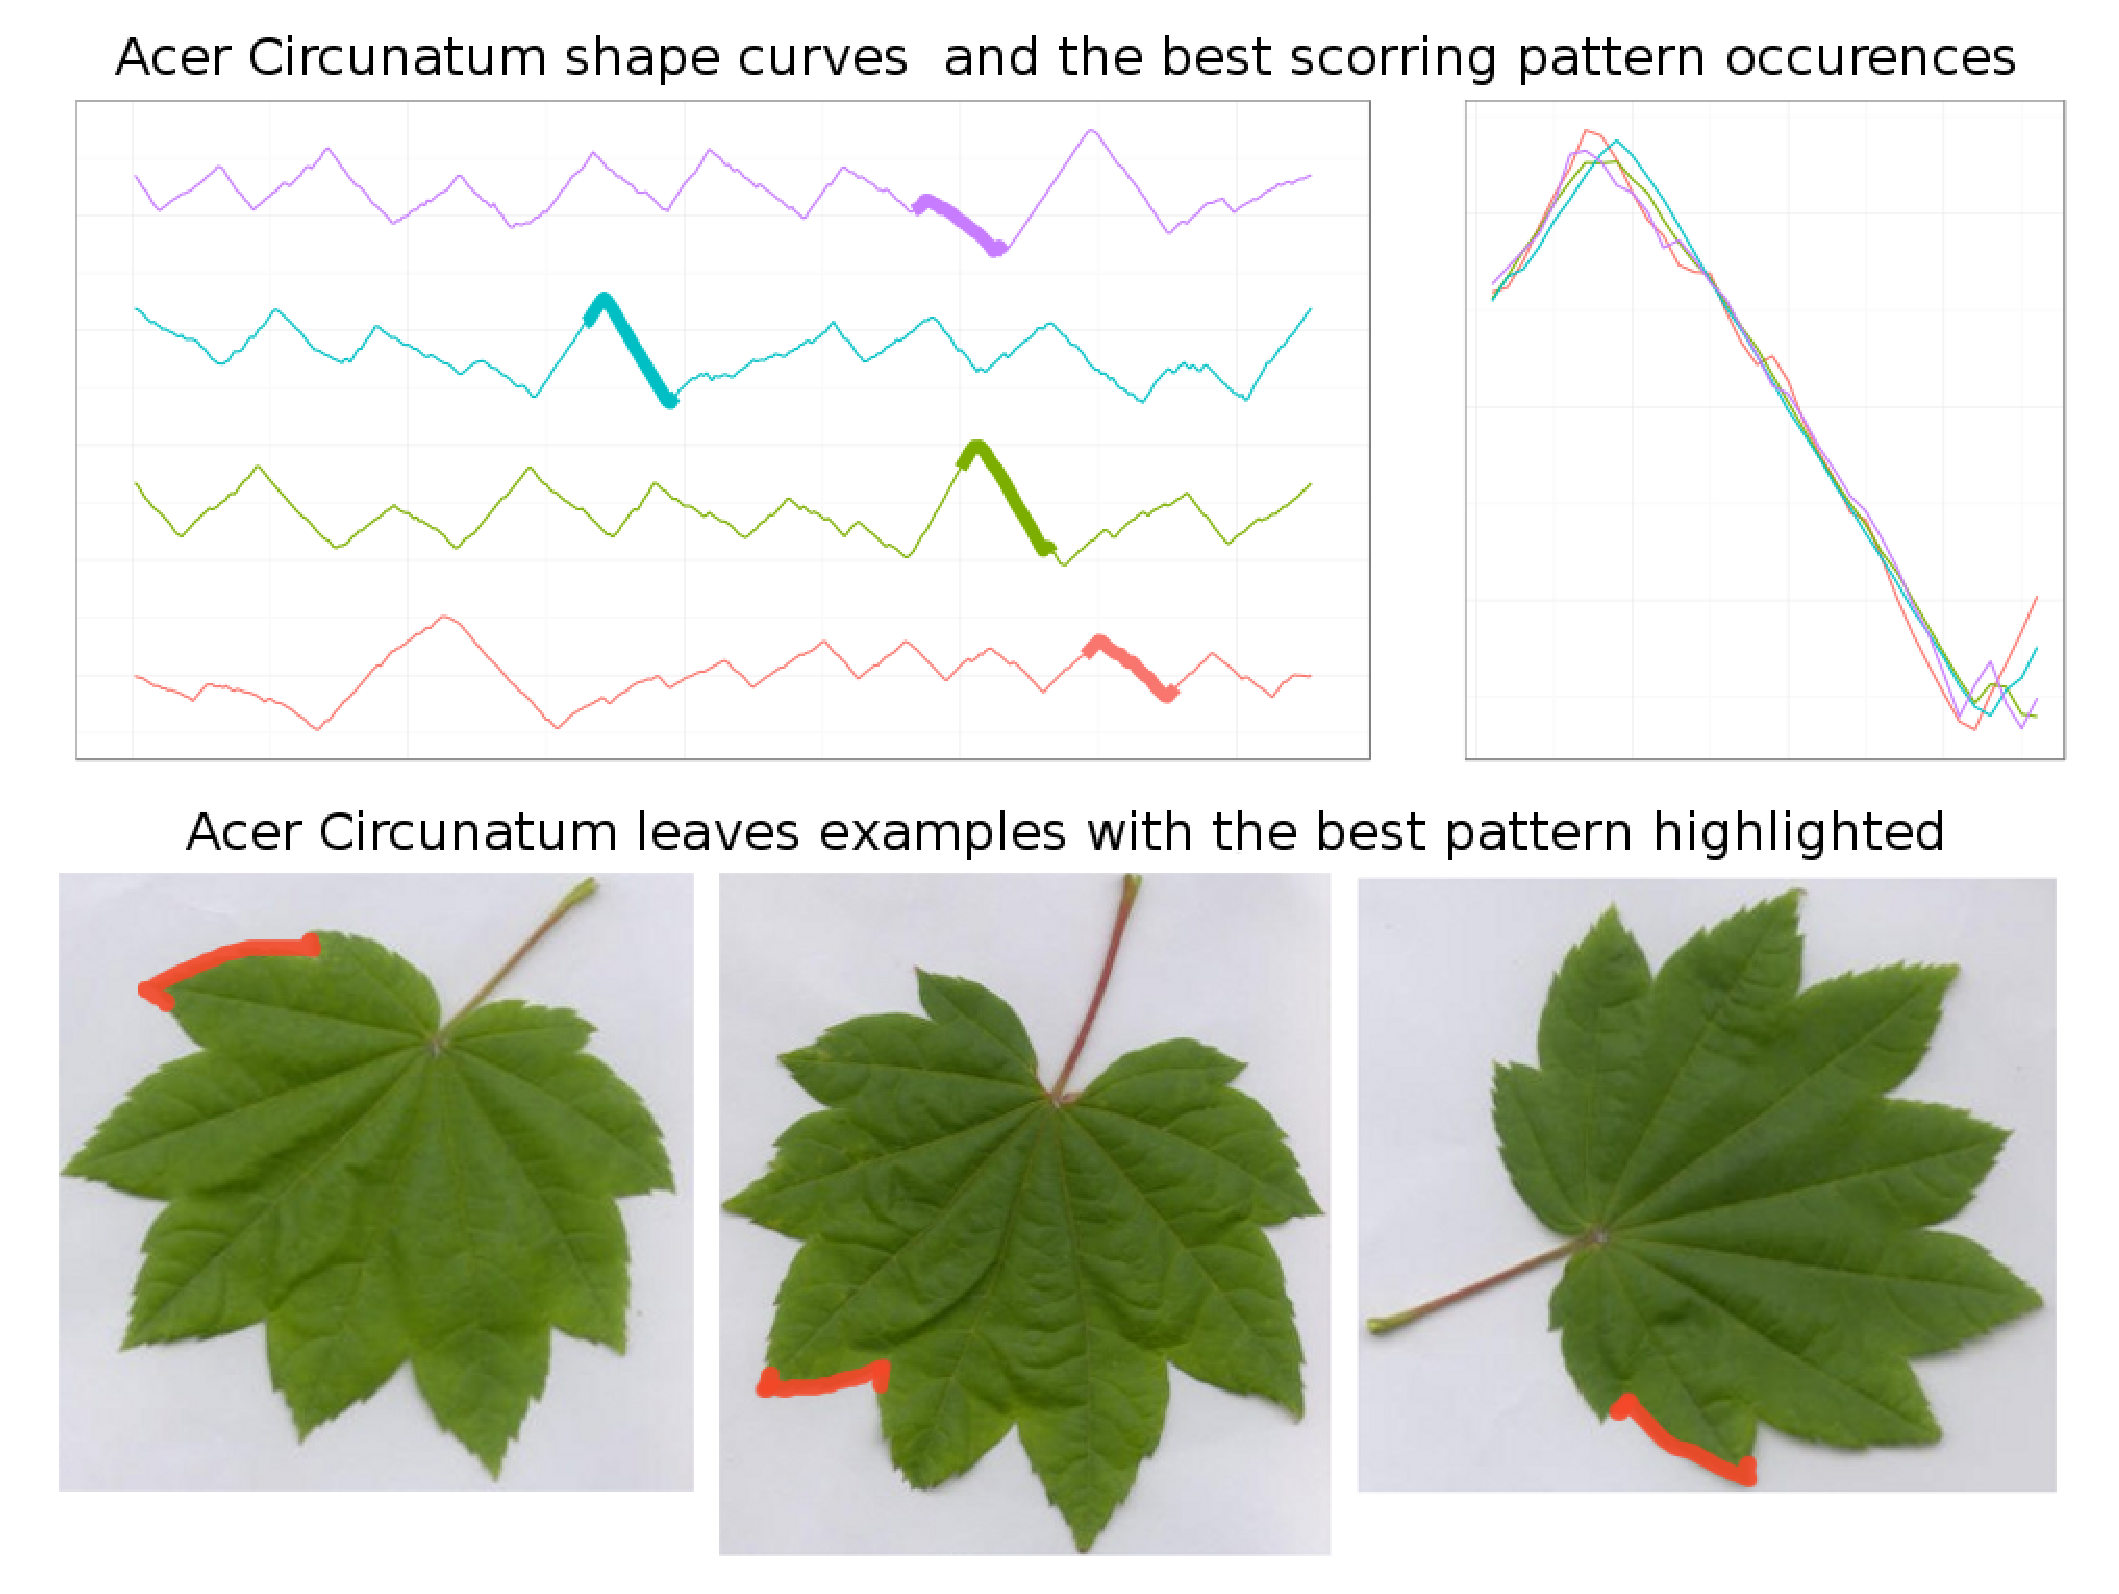
\includegraphics[width=140mm]{figures/AcerCircunatum.eps}
   \caption{Best characteristic subsequences (top panels, bold lines) discovered by SAX-VSM in
      \textit{OSULeaf data set}.
These patterns align with well known in botany discrimination techniques
by lobe shapes, serrations, and leaf tip types \cite{citeulike:12134192}.}
   \label{fig:shapelet-acer-patterns}
\end{figure}

\begin{figure}[t]
   \centering
   \includegraphics[width=140mm]{figures/coffee_patterns.ps}
   \caption{
   Best characteristic subsequences (left panels, bold lines) discovered by SAX-VSM in
   {Coffee data set}. Right panels show zoom-in view on these subsequences in Arabica
   and Robusta spectrograms.
   These discriminative subsequences correspond to chlorogenic acid (best subsequence) 
   and to caffeine (second to best) regions of spectra. This result aligns with
   the original work based on PCA \cite{citeulike:12550833} exactly.
   %Best characteristic subsequences discovered by SAX-VSM in \textit{Coffee data set}.
   %The best subsequences in both classes correspond to chlorogenic acid, while
   %second to best subsequences - to caffeine. This result aligns with previous 
   %exploratory research based on PCA \cite{citeulike:12550833}.
   }
   \label{fig:coffee}
\end{figure}

\subsubsection{Coffee data set}
Another illustration of interpretable classification with SAX-VSM is based on the analysis of its
performance on Coffee dataset \cite{citeulike:12550833}. The curves in this dataset correspond to spectra
obtained with diffuse reflection infrared Fourier transform (DRIFT) and truncated to 286 data points
in the region 800-1900 cm$^{-1}$. The two top-ranked by SAX-VSM subsequences in both datasets
correpond to spectrogram intervals of Chlorogenic acid (best) and Caffeine (second to best).
These two chemical compounds are known to be responsible for the flavor differences in 
Arabica and Robusta coffees; moreover, these spectrogram intervals were reported 
as discriminative when used in PCA-based technique by the authors of the original work
\cite{citeulike:12550833}.

\section{Clustering}
Clustering is a common tool used for data partitioning, visualization, exploration, and serves as
an important subroutine in many data mining algorithms. Typically, clustering algorithms
are built upon a distance function, and the overall performance of an algorithm is highly
dependent on a performance of the chosen function. Thus, an experimental evaluation of the 
proposed technique in clustering provides an additional perspective on its performance and
applicability beyond the classification.

\subsection{Hierarchical clustering}
Probably, one of the most used clustering algorithms is hierarchical clustering which requires no
parameters to be specified \cite{citeulike:1576606}. It computes pairwise distances between all objects and 
produces a nested hierarchy of clusters offering a great data visualization power. 

Previously, it was shown that the bag-of-patterns time series representation and Euclidean distance
provide a superior clustering performance\cite{citeulike:10525778}. 
For comparison, we performed similar experiments which differ in time series representation and
distance metric - we relied on $\text{\textbf{tf}}\ast\text{\textbf{idf}}$ weight vectors and cosine similarity. 
Affirming the previous work, we found, that the combination of SAX and Vector space model
outperforms classical shape-based distance metrics. 
For example, figure \ref{fig:hc} depicts the result of hierarchical clustering of a subset of
\textit{SyntheticControl} data. 
As one can see, SAX-VSM is superior in clustering performance to Euclidean and DTW distance 
metrics in this particular setup - it produced a hierarchy which properly partitions the
data set into three branches.

\subsection{k-Means clustering}
Another popular choice for data partitioning is k-Means clustering algorithm \cite{kmeans}.
The basic intuition behind this algorithm is that through the iterative reassignment of objects 
into different clusters the intra-cluster distance is minimized. As was shown, k-Means 
algorithm scales much better than hierarchical partitioning techniques \cite{citeulike:4195343}.
Fortunately, this clustering technique is well studied in IR field. Previously, in \cite{citeulike:505248}, the
authors extensively examined seven different criterion functions for partitional document
clustering and found, that \textit{k}-prototypes partitioning with cosine dissimilarity delivers an
excellent performance. 

Following this work, we implemented a similar to \cite{citeulike:1172599} \textit{spherical k-means algorithm}
and found, that algorithm converges quickly and delivers a satisfactory partitioning on short
synthetic data sets. Further, we evaluated our technique on the long time series from PhysioNet 
archive \cite{citeulike:699487}. 
We extracted two hundred fifty series corresponding to five vital signals: two ECG leads 
(aVR and II), and RESP, PLETH, and CO2 waves, trimming them to 2'048 points. Similarly to
\cite{citeulike:10525778}, we run a reference k-Means algorithm implementation based on Euclidean
distance, which achieved the maximum clustering quality of 0.39, when measured as proposed in
\cite{citeulike:1325189} on the best clustering (the one with the smallest objective function in 10 runs). 
SAX-VSM spherical k-Means implementation outperformed the reference technique yielding 
clusters  with the quality of 0.67 (on 10 runs with SAX parameters set to 
$W$=33, $P$=8, $A$=6).

%Note also, that previously, we applied our implementation to recurrent behaviors (motifs) 
%discovery in software development telemetry streams\cite{android}. 
%These behavioral time series were extracted from software change repositories and are 
%structurally similar to \textit{ElectricDevices} data set. 
%We used our \textit{tf$\ast$idf} weight vectors time series representation and spherical 
%k-Means implementation in order to discover specific temporal features corresponding 
%to the software release cycle. 
%Specifically, we optimized SAX parameters in order to obtain a proper partitioning of known 
%development behaviors before and after the software release. 
%In turn, the centroids of these clusters represented by \textit{tf$\ast$idf} weight vectors 
%were used to classify unlabeled  temporal intervals. 
%This technique allowed us to successfully classify pre- and post-release
%behaviors with accuracy above 80\%.

\begin{figure}[t]
   \centering
   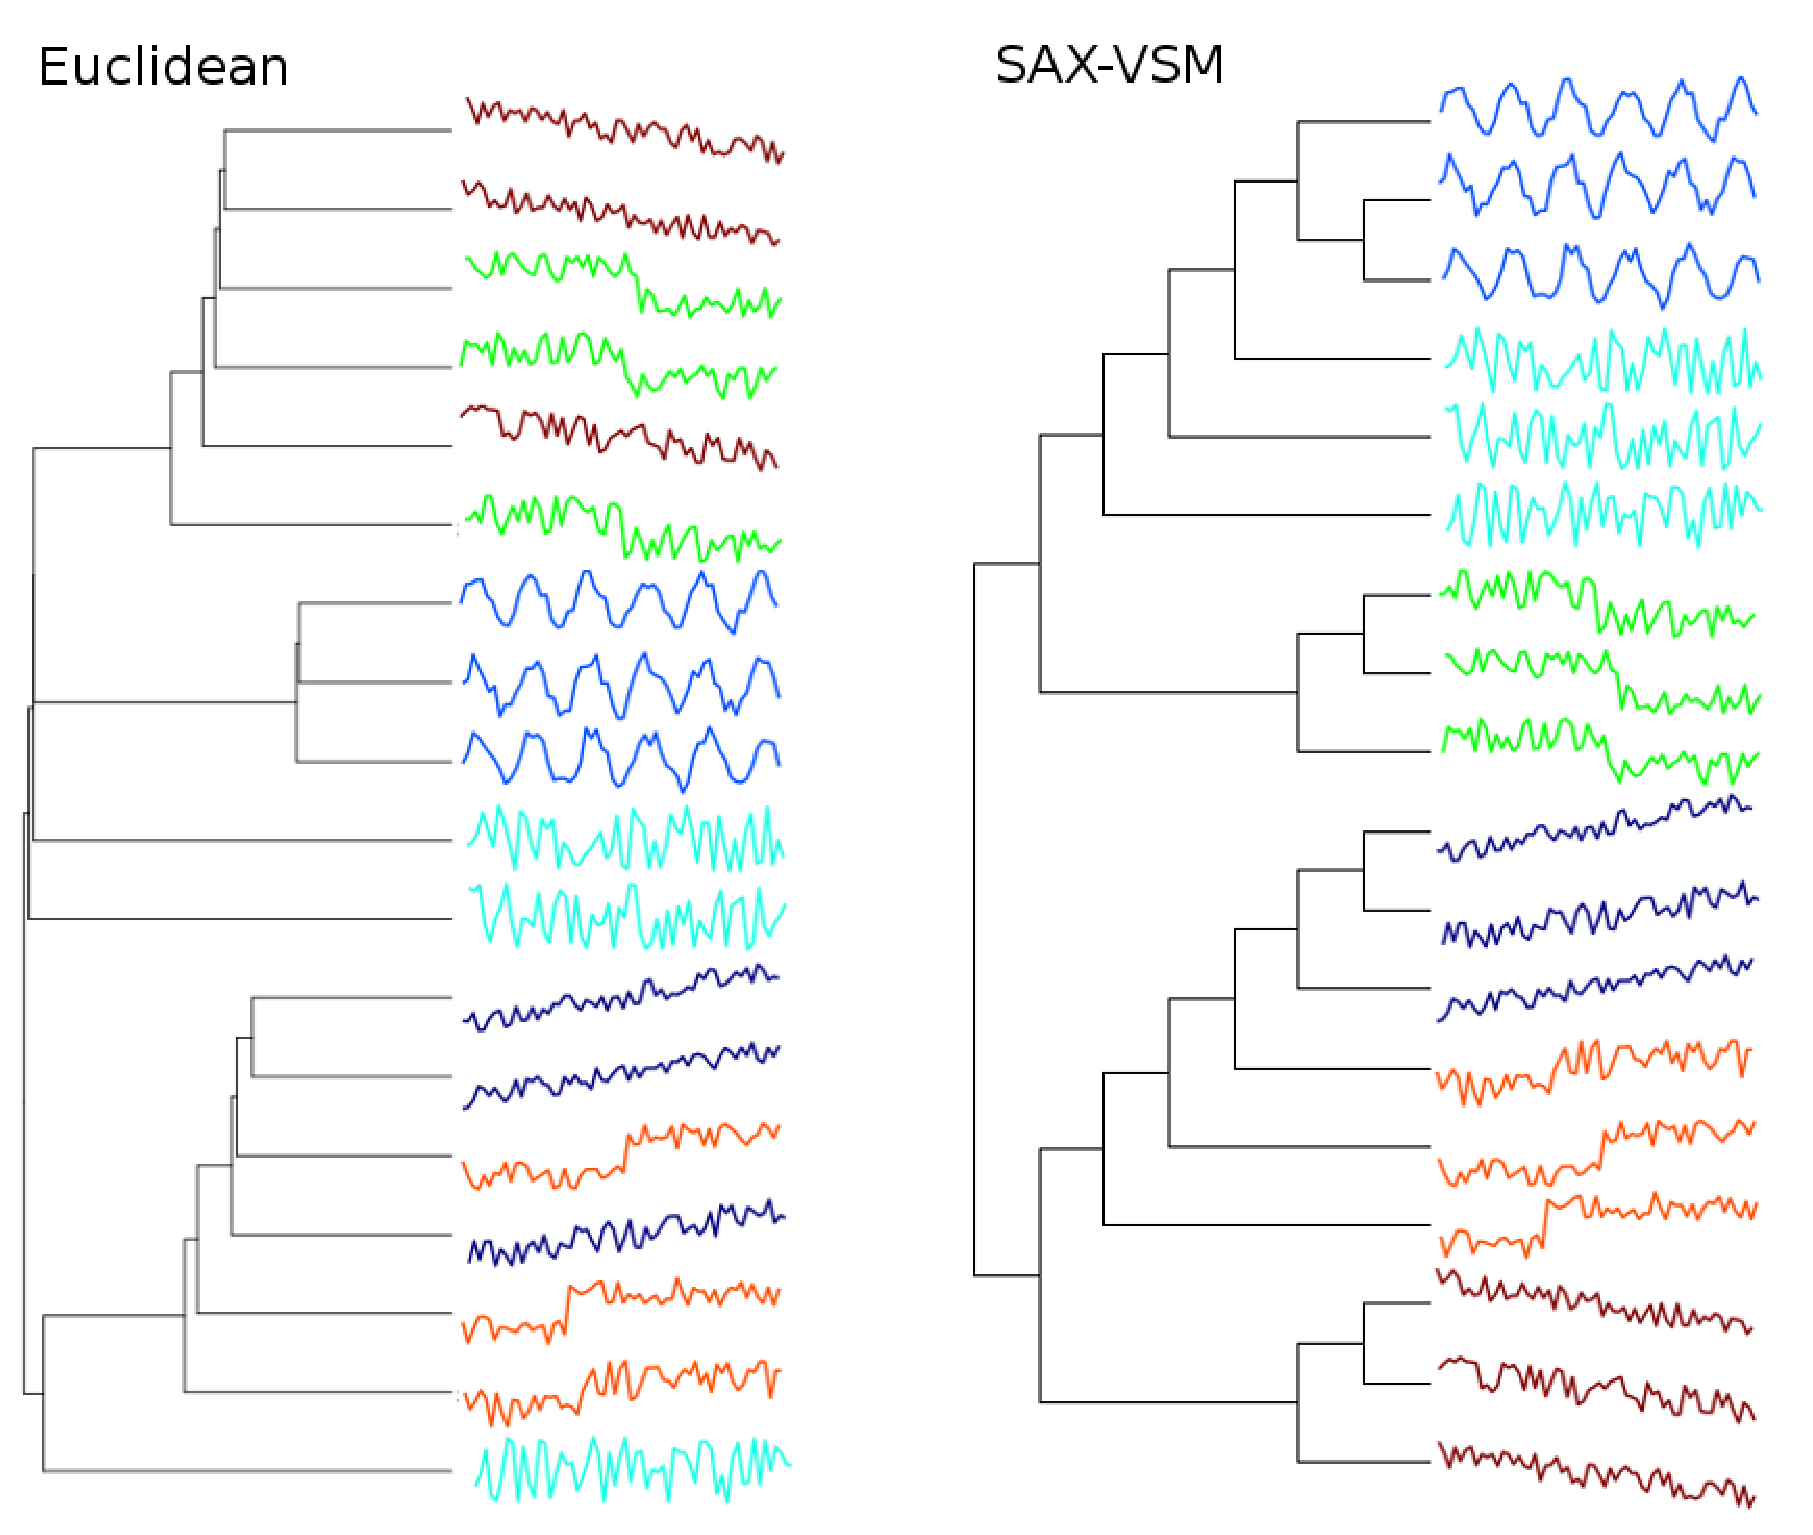
\includegraphics[width=140mm]{figures/clustering.eps}
   \caption{An comparison of hierarchical clustering application to a subset of three
   \textit{SyntheticControl} classes: \textit{Normal, Decreasing trend}, and \textit{Upward shift}. 
   Euclidean distance, Dynamic time warping, SAX-VSM and Complete linkage were used to 
   generate these plots. Only SAX-VSM was able to partition series properly.                       
   }
   \label{fig:hc}
\end{figure}

\section{Conclusion and Future Work} \label{conclusion}
In this paper, we have proposed a novel interpretable technique for time series classification
based on characteristic patterns discovery. We have shown, that our approach is competitive with, 
or superior to, other techniques on a variety of classic data mining problems. In addition, 
we described several advantages of SAX-VSM over existing structure-based similarity measures,
emphasizing its capacity to discover and rank short subsequences by their class characterization
power.

The current limitations of our SAX-VSM implementation suggest a number of future work directions. 
First of all, while Vector space model naturally supports processing of bags of words composed 
of terms of variable length, our current ``stable'' implementation lacks this capacity.
Inspired by the recently reported superior performance of multi-shapelets based classifiers
\cite{citeulike:11345338}, we prioritize this development.
Secondly, as mentioned before, DIRECT optimization it is designed for a function of a real variable.
By using rounding in our implementation, we have observed DIRECT iteratively sampling redundant
locations in suboptimal neighborhood, thus, a more appropriate optimization scheme is needed.
Finally, we are designing and experimenting with an extension of SAX-VSM to multidimensional time
series. Currently we are evaluating two candidate implementations: the first is based on a
single bag of words accommodating all dimensions for a class (by prefixing SAX words extracted from
different dimensions); while the second is based on the use of a single bag of words per each of
dimensions. The preliminary results on synthetic data sets look promising and we expect to report 
our finding soon.
